\setAuthor{Erkki Tempel}
\setRound{piirkonnavoor}
\setYear{2023}
\setNumber{G 6}
\setDifficulty{6}
\setTopic{TODO}

\prob{Klaasplaat}
\begin{wrapfigure}{r}{0.3\textwidth}
  \vspace{-2em}
  \begin{center}
    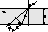
\includegraphics[width=1\linewidth]{2023-v2g-06-yl.pdf}
    %\caption{}
  \end{center}
  \vspace{-2em}
\end{wrapfigure}

Leidke, kui palju nihkub valguskiir kõrvale esialgse sihi suhtes pärast klaasplaadi läbimist. Kiire langemisnurk on $\alpha$, klaasi murdumisnäitaja on $n$ ning klaasplaadi paksus on $d$. Täispunktide saamiseks palume vastuses mitte kasutada trigonomeetrilisi pöördfunktsioone (nt $\arcsin$, $\arccos$).


\hint

\solu
\begin{center}
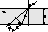
\includegraphics[width=0.5\linewidth]{2023-v2g-06-sol.pdf}
\end{center}
  
Kolmnurgast $\triangle{ABC}$ saame avaldada kiire nihke $BC$\\
\[ BC = AC \cos{\alpha} \quad \p{2}\]

Külje $AC$ pikkuse saame leida lõikude $AD$ ja $CD$ kaudu
\[ AC = AD - CD  \quad \p{1}\]

Avaldame külje AD kolmnurgast $\triangle{ADE}$
\[ AD = d\tan{\alpha} \quad \p{1}\]
Külje CD leidmiseks kasutame murdumisnäitaja seost
\[ \frac{\sin{\alpha}}{\sin{\gamma}} = n \quad \Longrightarrow \quad \sin{\gamma} = \frac{\sin{\alpha}}{n} \quad   \p{1}\]
Kolmnurgast  $\triangle{CDE}$ saame avaldada $\sin{\gamma}$ ning sealt külje $CD$
\[ \sin{\gamma} = \frac{CD}{CE} \quad \Longrightarrow \quad  CD = \frac{CE \sin{\alpha}}{n} \quad\p{1}\]

Kasutades eelnevat seost ning Phytagorase teoreemi kolmnurgast $\triangle{CDE}$,
saame avaldada külje CD
\[  CD = \frac{d\sin{\alpha}}{\sqrt{n^2-\sin^2{\alpha}}} \quad \p{2}  \]

Seega nihkub esialgne kiir kõrvale oma algsest sihist 

\[ BC = d\sin{\alpha}\left(1 - \frac{\cos{\alpha}}{\sqrt{n^2-\sin^2{\alpha}}}\right)  \quad \p{2}  \]

Kui lõppvastusesse on jäetud lihtsustamata trigonomeetriline pöördfunktsioon (nt $\arcsin$, $\arccos$), siis anda ülesande eest kuni \p{8}.
\probend